% LLM-YARA — Specificity Comparison Horizontal Bar Chart
% Compile: pdflatex specificity_comparison.tex
\documentclass[border=5pt]{standalone}
\usepackage{tikz}
\usepackage{pgfplots}
\pgfplotsset{compat=1.18}

% ── Colour palette ──────────────────────────────────────────────────
\definecolor{hlblue}{HTML}{2563EB}
\definecolor{hlbluefill}{HTML}{93C5FD}
\definecolor{bardgray}{HTML}{94A3B8}
\definecolor{bardgrayfill}{HTML}{CBD5E1}
\definecolor{txtgray}{HTML}{374151}
\definecolor{perfgreen}{HTML}{16A34A}

\begin{document}
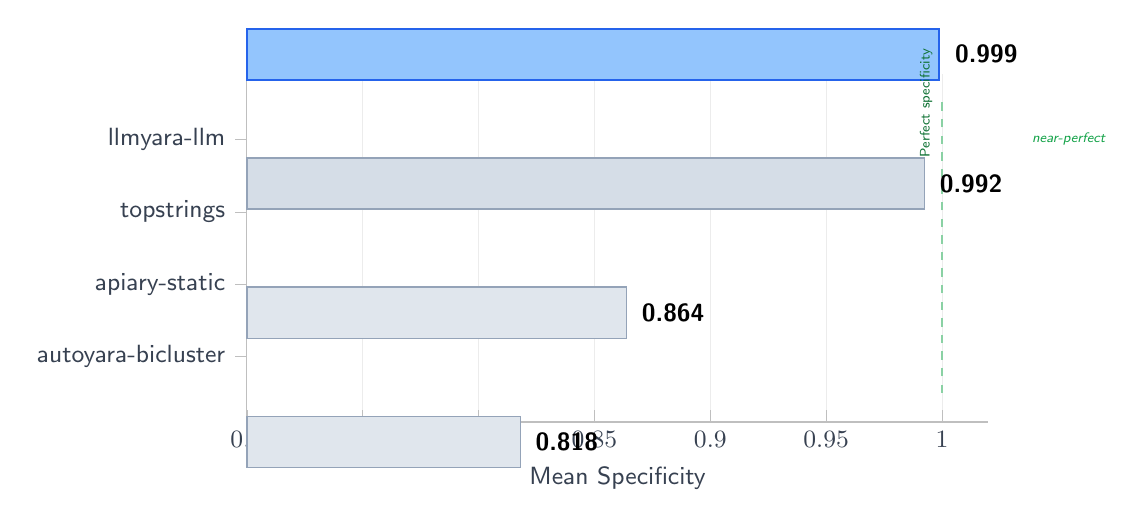
\begin{tikzpicture}
\begin{axis}[
    xbar,
    width=11cm,
    height=6cm,
    bar width=0.65cm,
    xmin=0.70, xmax=1.02,
    ytick={1, 2, 3, 4},
    yticklabels={
        {autoyara-bicluster},
        {apiary-static},
        {topstrings},
        {llmyara-llm}},
    y tick label style={font=\sffamily\small, text=txtgray, anchor=east},
    x tick label style={font=\sffamily\small, text=txtgray,
        /pgf/number format/fixed, /pgf/number format/precision=2},
    xtick={0.70, 0.75, 0.80, 0.85, 0.90, 0.95, 1.00},
    xlabel={Mean Specificity},
    xlabel style={font=\sffamily\small, text=txtgray},
    xmajorgrids=true,
    grid style={gray!15, thin},
    axis line style={gray!50},
    tick style={gray!50},
    axis x line*=bottom,
    axis y line*=left,
    enlarge y limits=0.3,
    clip=false,
    nodes near coords,
    nodes near coords align={horizontal},
    every node near coord/.append style={
        font=\sffamily\small\bfseries,
        anchor=west,
        xshift=2pt,
    },
    point meta=explicit symbolic,
]

% ── autoyara-bicluster ──────────────────────────────────────────────
\addplot[
    fill=bardgrayfill!60, draw=bardgray, line width=0.5pt,
] coordinates {
    (0.817978, 1) [0.818]
};

% ── apiary-static ──────────────────────────────────────────────────
\addplot[
    fill=bardgrayfill!60, draw=bardgray, line width=0.5pt,
] coordinates {
    (0.863839, 2) [0.864]
};

% ── topstrings ──────────────────────────────────────────────────────
\addplot[
    fill=bardgrayfill!80, draw=bardgray, line width=0.5pt,
] coordinates {
    (0.992386, 3) [0.992]
};

% ── llmyara-llm (highlighted) ──────────────────────────────────────
\addplot[
    fill=hlbluefill, draw=hlblue, line width=0.7pt,
] coordinates {
    (0.998832, 4) [0.999]
};

% ── Near-perfect annotation ─────────────────────────────────────────
\node[font=\sffamily\tiny\itshape, text=perfgreen, anchor=west]
    at (axis cs:0.998832, 4) [xshift=30pt, yshift=0pt]
    {near-perfect};

% ── Vertical reference line at 1.0 ─────────────────────────────────
\draw[perfgreen!50, dashed, line width=0.6pt]
    (axis cs:1.0, 0.5) -- (axis cs:1.0, 4.6);
\node[font=\sffamily\tiny, text=perfgreen!70!black, anchor=south, rotate=90]
    at (axis cs:1.0, 4.5) [xshift=0pt] {Perfect specificity};

\end{axis}
\end{tikzpicture}
\end{document}
